\documentclass[a4paper,12pt]{article}

\usepackage{titling}
\usepackage{amsmath}
\usepackage{graphicx}
%\usepackage[showframe=true]{geometry}
\usepackage{changepage}

\begin{document}

\title{Distributed Computing - Final Architecture Coltivate - Group 4}
\author{ Rafael De Smet \\
  \texttt{rafael.desmet@student.uantwerpen.be}  \and
  Keerthana Sanala Prakash \\
  \texttt{keerthana.sanalaprakash@student.uantwerpen.be} \and
  Jordan Parezys \\
  \texttt{jordan.parezys@student.uantwerpen.be}}
\date{}
\maketitle

\section{Introduction}

In this document we explain the architecture of our website. We give a schematic overview and a detailed explanation of all the services in our system. The website contains the mandatory services as requested in the assignment and also some extra services, asked for by the students of the Persuasive Technology course. The goal of the website is to create a platform that allows users to exchange homegrown vegetables and fruits, named Coltivate.

\section{Microservices}

All the communication between the microservices is done via the REST protocol. Two users that chat communicate via websockets. In the front-end of all the services, we give the user the options to at any time go to either the chat, his garden page, the map with other users or to make a new post.

\subsection{Admin Service}

TODO

\subsection{Advertising Service}

This service handles the advertisements. It is linked to the post service and to the newsfeed service. When a new post is made by the current user, we sent this information to the advertisement service. Here we see what the user posted about. If he mentioned for example that he is growing potatoes, the service will select an advertisement about potatoes. Likewise with other vegetables, fruits and herbs.
\newline

The chosen advertisements are sent to the newsfeed to display it to the user. This service has its own separate database to store the advertisements. Only an admin can add or remove advertisements.

\subsection{Chat Service}

The chat service is implemented as a standalone application aswell as an integrated part of the website. It is implemented based on websockets that talk to each other privately. When a user goes to the chat app, he sees a list of users he can chat with. You don't have to be friends with another user to be able to chat with each other. When user Alice sees that user Bob has some products she might be interested in, she want to directly chat with Bob, instead of having to befriend him first.

\subsection{Comment Service}

The comment service is linked with the post service and stores all the comments users made on the posts that are on the newsfeed. In the newsfeed there is per post a textarea provided to easily leave a comment on a post. The newsfeed service sends the new comment to the comment service where it is stored together with information about the post it belongs to. When a user wants to leave a comment on a post, we first check with the cyber bully service whether it is allowed or not. 

\subsection{Cyber Bullying Service}

This is a mandatory service which receives the text of a new post or of a new comment. We have provided two lists of English and Dutch words that may be considered rude or not fit on a website. When a bad word from the list is seen in the post or comment, we let the correct service know. In this case the user gets a message warning him that he used a bad word. The option is given to discard the comment or post, or to submit it anyway.

\subsection{Garden Service}

In the idea of Coltivate, every user has its own garden, where they can add new vegetables, fruits or herbs. Other users can visit this page to see the produce someone else has. The page is divided in four tabs, one showing the whole garden, one showing only the vegetables, one only the fruits and one only the herbs. A separate page is provided where the user can add new produce. The possible produce a user can use is stored in the separate database.

\subsection{Location Service}

This service was not in the original scope of the assignment, but was requested by the PT group. This service uses a Google Maps API to show a map where all the other users of the website are located. When a user goes to this page, he sees information about the garden of all the users around him. Therefore this service is linked to the garden service. Should a user be interested to chat immediately with another user he sees on the map, he can do so by clicking on the provided button (for each user). Analogously if he wants to become friends with another user. The addresses of all the users are retrieved from the user service.

\subsection{Login/Registration and User Service}

This service stores all information about the users registered on the website. If a user surfs to the website he is asked to login, then is automatically redirected to his newsfeed. Should a new user arrive who is not yet registered, he can fill in his information and register. Besides his name and email, we also ask him the address of his garden. This address is used to be able to show him in the map of the location service. In the User database we store all the users registered on the website. An admin user is also stored here, denoted by a Boolean column in the database. Besides the user information, we also store the Friendship information here. Two users can be friends with each other, if so this information is stored here.
\newline

This service is linked to a few other services, such as the newsfeed, the garden, the location and the chat. These services can only be accessed when a user is logged in and they also need to know the information about the current user. We send the user id via the session cookie with which they then can ask other information about the user if needed. 

\subsection{Newsfeed Service}

The newsfeed collects all the latest posts and comments that belong to those posts, the latest photos and the current advertisements suited for the user. All this is shown in a list. This service is linked to the post, comment, photo, advertisement, notifications and chat services.

\subsection{Post Service}

This service handles the submission of new posts and photos. When a user want to submit a post to the newsfeed, we first check with the cyber bully service whether it is allowed or not. If it is allowed, we submit it straight away. When it is not allowed, we let the user know and give him the choice to discard or submit anyway. All the text posts are stored here. When a user wants to upload a photo, we sent this new photo to the photo service to store it there.

\begin{adjustwidth}{-3cm}{}
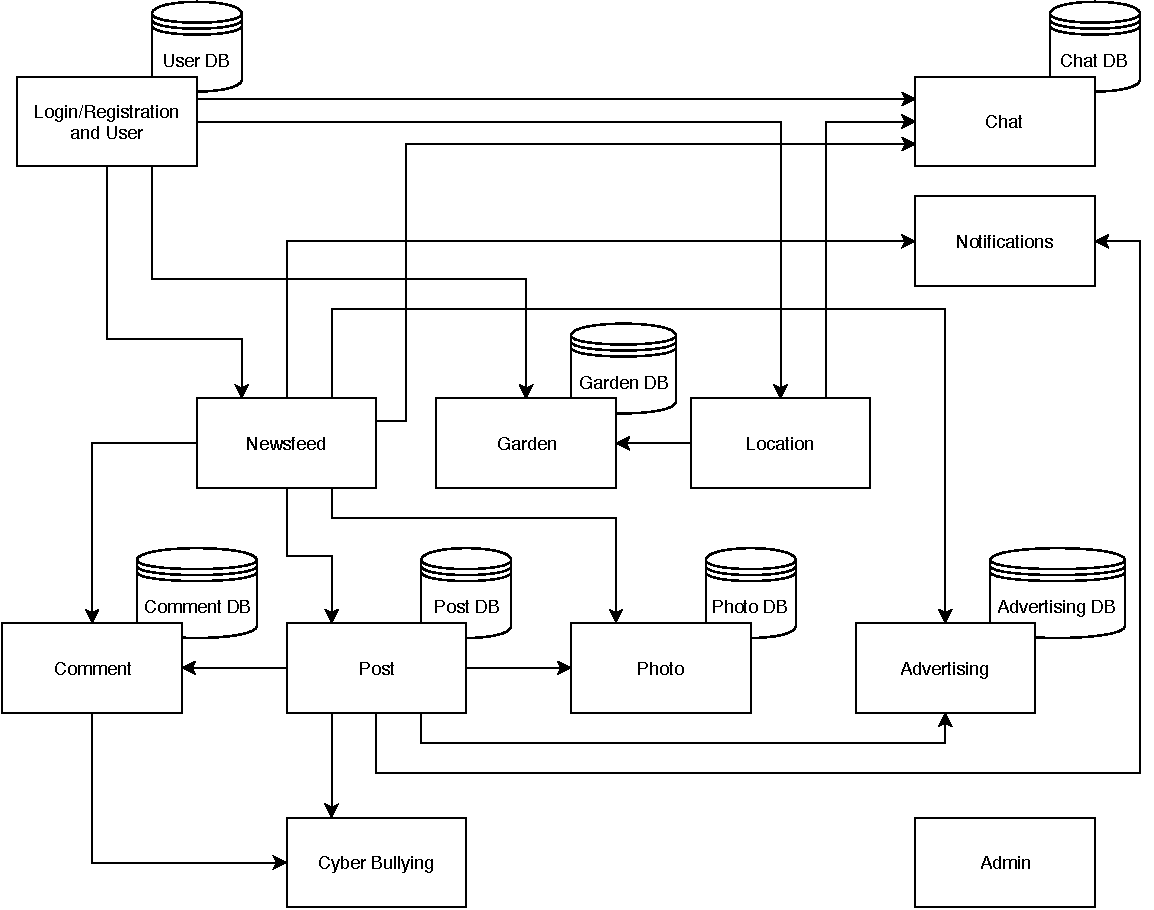
\includegraphics[scale=1]{Microservices_architecture_final.pdf} 
\end{adjustwidth}

\end{document}
